\subsubsection{Ý tưởng}
Radix Sort là một thuật toán sắp xếp không dựa trên so sánh, hoạt động dựa trên các chữ số của phần tử trong mảng. Thuật toán xử lý các phần tử theo từng chữ số (bắt đầu từ chữ số hàng đơn vị, sau đó đến hàng chục, hàng trăm, v.v.). Ở mỗi bước, các phần tử được sắp xếp cục bộ bằng một thuật toán sắp xếp ổn định như Counting Sort.

\subsubsection{Mã giả}

\begin{algorithm}[H]
\caption{Radix Sort}
\begin{algorithmic}[1]
\Procedure{RadixSort}{$arr, n$}
    \State \textbf{Input:} Mảng $arr$ gồm $n$ phần tử
    \State \textbf{Output:} Mảng $arr$ được sắp xếp
    
    \State Tìm giá trị lớn nhất trong $arr$: $max \gets \max(arr)$
    
    \State Khởi tạo $exp \gets 1$ \Comment{Biểu thị chữ số cần xét: 1, 10, 100, ...}
    \While{$max / exp > 0$}
        \State \Call{CountingSort}{$arr, n, exp$} \Comment{Sắp xếp theo chữ số hiện tại}
        \State $exp \gets exp \times 10$
    \EndWhile
\EndProcedure

\Procedure{CountingSort}{$arr, n, exp$}
    \State \textbf{Input:} Mảng $arr$ gồm $n$ phần tử, chữ số cần xét $exp$
    \State \textbf{Output:} Mảng $arr$ được sắp xếp theo chữ số hàng $exp$
    
    \State Khởi tạo mảng đếm $count[0..9] \gets 0$
    \State Khởi tạo mảng tạm $output[1..n]$
    
    \State \textbf{Đếm số lần xuất hiện:}
    \For{$i \gets 1$ \textbf{to} $n$}
        \State $digit \gets \lfloor arr[i] / exp \rfloor \mod 10$
        \State $count[digit] \gets count[digit] + 1$
    \EndFor
    
    \State \textbf{Tính chỉ số thực tế:}
    \For{$i \gets 1$ \textbf{to} $9$}
        \State $count[i] \gets count[i] + count[i-1]$
    \EndFor
    
    \State \textbf{Sắp xếp phần tử theo chữ số hiện tại:}
    \For{$i \gets n$ \textbf{down to} $1$}
        \State $digit \gets \lfloor arr[i] / exp \rfloor \mod 10$
        \State $output[count[digit]] \gets arr[i]$
        \State $count[digit] \gets count[digit] - 1$
    \EndFor
    
    \State \textbf{Cập nhật mảng ban đầu:}
    \For{$i \gets 1$ \textbf{to} $n$}
        \State $arr[i] \gets output[i]$
    \EndFor
\EndProcedure
\end{algorithmic}
\end{algorithm}

\subsubsection{Ví dụ}

Giả sử chúng ta có mảng ban đầu: $[38, 27, 43, 3, 9, 82, 10]$. Dưới đây là các bước thực hiện Radix Sort minh họa bằng hình ảnh:

\begin{enumerate}
    \item Tạo mảng đếm và mảng phụ để lưu trữ kết quả trung gian:
    \begin{figure}[H]
        \centering
        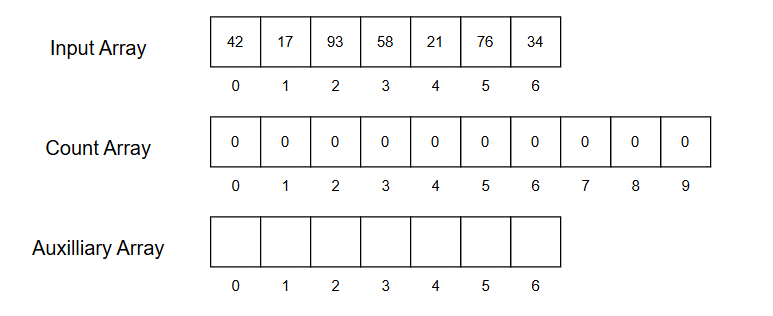
\includegraphics[width=0.7\textwidth]{img/radix_sort/1.png}
        \caption{Minh họa RadixSort-1}
    \end{figure}
    
    \item Đếm số lần xuất hiên của chứ số hàng đơn vị và lưu vào mảng đếm:
    \begin{figure}[H]
        \centering
        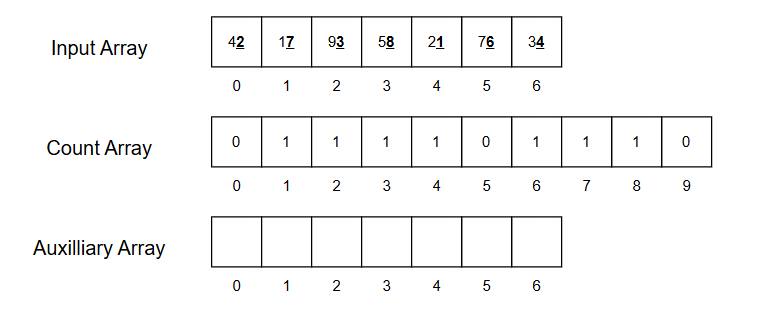
\includegraphics[width=0.7\textwidth]{img/radix_sort/2.png}
        \caption{Minh họa RadixSort-2}
    \end{figure}
    
    \item Thực hiện cộng dồn ở mảng đến và trừ mỗi phần tử ở mảng đếm đi 1 để tính chỉ số của phần tử trong mảng kết quả:
    \begin{figure}[H]
        \centering
        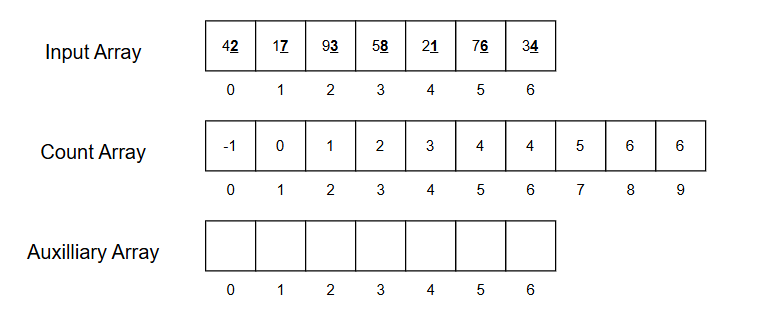
\includegraphics[width=0.7\textwidth]{img/radix_sort/3.png}
        \caption{Minh họa RadixSort-3}
    \end{figure}
    
    \item Duyệt mảng ban đầu từ cuối về đầu, lưu từng phần tử vào mảng kết quả tạm thời với chỉ số là giá trị trong mảng count ứng với chữ số hàng đơn vị của phần tử đó:
    \begin{figure}[H]
        \centering
        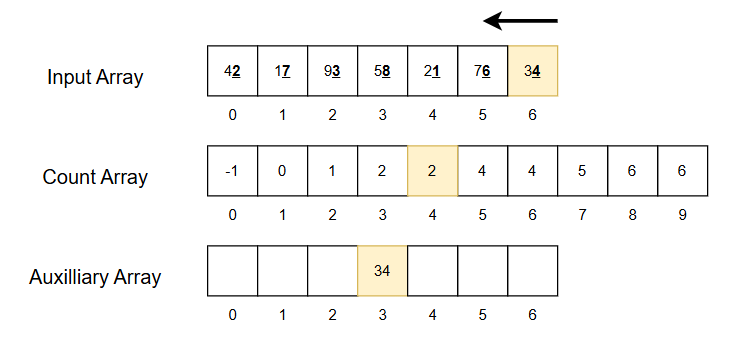
\includegraphics[width=0.7\textwidth]{img/radix_sort/4.png}
        \caption{Minh họa RadixSort-4}
    \end{figure}
    
    \item Kết thúc bước sắp xếp chữ số hàng đơn vị:
    \begin{figure}[H]
        \centering
        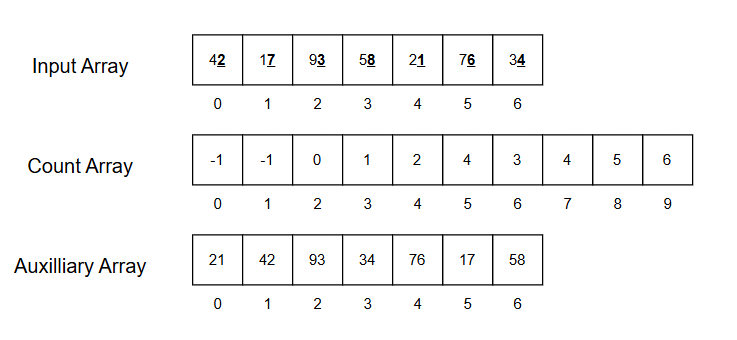
\includegraphics[width=0.7\textwidth]{img/radix_sort/5.png}
        \caption{Minh họa RadixSort-5}
    \end{figure}
    
    \item Cập nhật mảng ban đầu với mảng kết quả tạm thời:
    \begin{figure}[H]
        \centering
        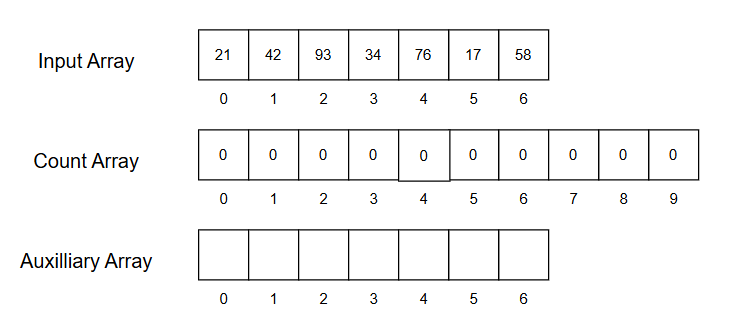
\includegraphics[width=0.7\textwidth]{img/radix_sort/6.png}
        \caption{Minh họa RadixSort-6}
    \end{figure}
    
    \item Đếm số lần xuất hiên của chứ số hàng chục và lưu vào mảng đếm:
    \begin{figure}[H]
        \centering
        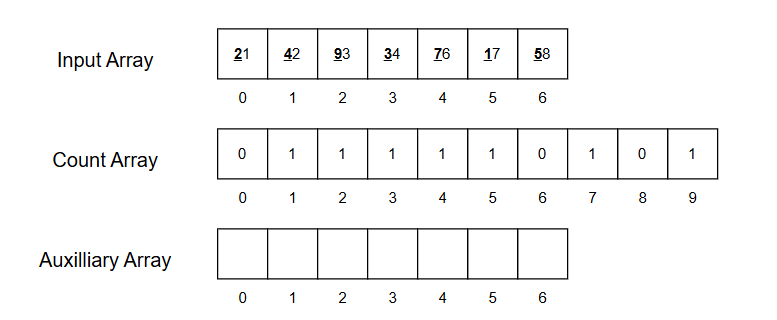
\includegraphics[width=0.7\textwidth]{img/radix_sort/7.png}
        \caption{Minh họa RadixSort-7}
    \end{figure}
    
    \item Thực hiện cộng dồn ở mảng đến và trừ mỗi phần tử ở mảng đếm đi 1 để tính chỉ số của phần tử trong mảng kết quả:
    \begin{figure}[H]
        \centering
        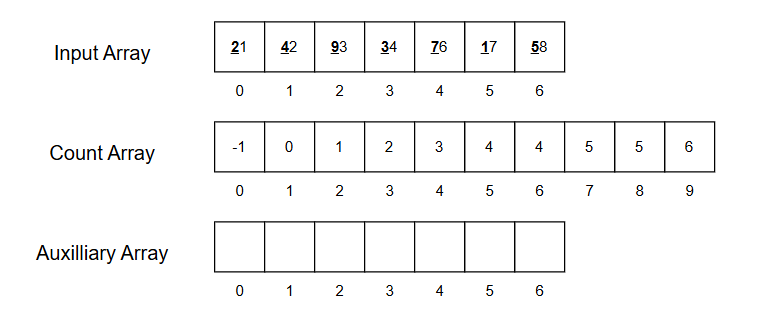
\includegraphics[width=0.7\textwidth]{img/radix_sort/8.png}
        \caption{Minh họa RadixSort-8}
    \end{figure}
    
    \item Duyệt mảng ban đầu từ cuối về đầu, lưu từng phần tử vào mảng kết quả tạm thời với chỉ số là giá trị trong mảng count ứng với chữ số hàng chục của phần tử đó:
    \begin{figure}[H]
        \centering
        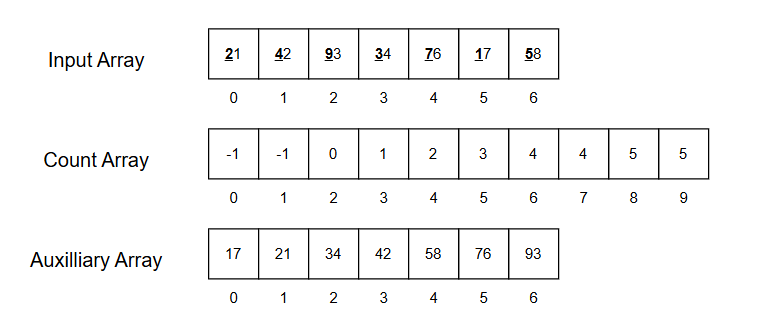
\includegraphics[width=0.7\textwidth]{img/radix_sort/9.png}
        \caption{Minh họa RadixSort-9}
    \end{figure}
    
    \item Hoành thành sắp xếp:
    \begin{figure}[H]
        \centering
        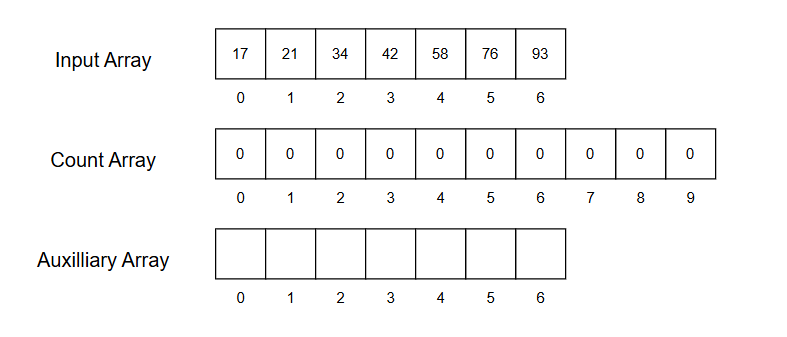
\includegraphics[width=0.7\textwidth]{img/radix_sort/10.png}
        \caption{Minh họa RadixSort-10}
    \end{figure}
\end{enumerate}

\subsubsection{Độ phức tạp}
\begin{itemize}
    \item[\textbf{--}] \textbf{Thời gian:}
    \begin{itemize}
        \item[$\bullet$] Sắp xếp mỗi chữ số cần \(\mathcal{O}(n + k)\), trong đó:
        \begin{itemize}
            \item \(n\) là số lượng phần tử trong mảng.
            \item \(k\) là số lượng giá trị có thể xuất hiện (thông thường \(k = 10\), tương ứng với các chữ số từ 0 đến 9).
        \end{itemize}
        \item[$\bullet$] Tổng số chữ số cần xử lý là \(d = \lfloor \log_b(\text{max}) \rfloor + 1\), trong đó \(b\) là cơ số (ở đây \(b = 10\)).
        \item[$\bullet$] Vì vậy, tổng thời gian thực hiện là:
        \[
        \mathcal{O}(d \cdot (n + k))
        \]
        \item[$\bullet$] Với \(k\) là hằng số, độ phức tạp có thể rút gọn thành \(\mathcal{O}(d \cdot n)\).
    \end{itemize}
    \item[\textbf{--}] \textbf{Không gian:}
    \begin{itemize}
        \item[$\bullet$] Bộ nhớ tạm cần thiết bao gồm:
        \begin{itemize}
            \item \(\mathcal{O}(n)\) cho mảng tạm \(output\) để lưu trữ kết quả trung gian.
            \item \(\mathcal{O}(k)\) cho mảng đếm \(count\).
        \end{itemize}
        \item[$\bullet$] Tổng không gian bộ nhớ: \(\mathcal{O}(n + k)\).
    \end{itemize}
    \item[\textbf{--}] \textbf{Tính ổn định:}
    \begin{itemize}
        \item[$\bullet$] Radix Sort là một thuật toán \textbf{ổn định} nếu Counting Sort trong từng bước xử lý chữ số được triển khai theo cách ổn định. Tính ổn định đảm bảo rằng thứ tự ban đầu của các phần tử có giá trị bằng nhau trong mảng sẽ không thay đổi sau khi sắp xếp.
    \end{itemize}
\end{itemize}